% This file was created with tikzplotlib v0.10.1.
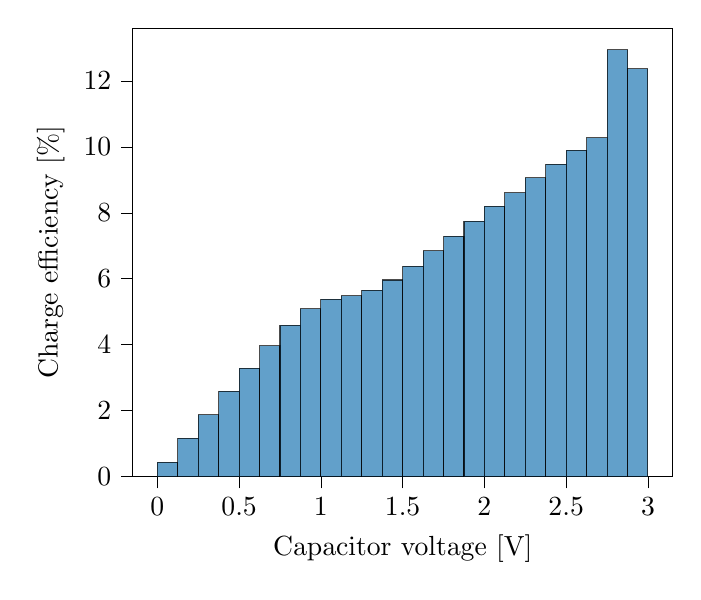
\begin{tikzpicture}

\definecolor{darkgray176}{RGB}{176,176,176}
\definecolor{steelblue31119180}{RGB}{31,119,180}

\begin{axis}[
tick align=outside,
tick pos=left,
x grid style={darkgray176},
xlabel={Capacitor voltage [V]},
xmin=-0.15, xmax=3.15,
xtick style={color=black},
y grid style={darkgray176},
ylabel={Charge efficiency [\%]},
ymin=0, ymax=13.5999914762888,
ytick style={color=black}
]
\draw[draw=black,fill=steelblue31119180,opacity=0.7] (axis cs:0,0) rectangle (axis cs:0.125,0.428298634962978);
\draw[draw=black,fill=steelblue31119180,opacity=0.7] (axis cs:0.125,0) rectangle (axis cs:0.25,1.15440254145031);
\draw[draw=black,fill=steelblue31119180,opacity=0.7] (axis cs:0.25,0) rectangle (axis cs:0.375,1.87665213771732);
\draw[draw=black,fill=steelblue31119180,opacity=0.7] (axis cs:0.375,0) rectangle (axis cs:0.5,2.58404915625955);
\draw[draw=black,fill=steelblue31119180,opacity=0.7] (axis cs:0.5,0) rectangle (axis cs:0.625,3.28025015092578);
\draw[draw=black,fill=steelblue31119180,opacity=0.7] (axis cs:0.625,0) rectangle (axis cs:0.75,3.96436953632097);
\draw[draw=black,fill=steelblue31119180,opacity=0.7] (axis cs:0.75,0) rectangle (axis cs:0.875,4.5860301309526);
\draw[draw=black,fill=steelblue31119180,opacity=0.7] (axis cs:0.875,0) rectangle (axis cs:1,5.09162445857025);
\draw[draw=black,fill=steelblue31119180,opacity=0.7] (axis cs:1,0) rectangle (axis cs:1.125,5.38308278858274);
\draw[draw=black,fill=steelblue31119180,opacity=0.7] (axis cs:1.125,0) rectangle (axis cs:1.25,5.49122732060493);
\draw[draw=black,fill=steelblue31119180,opacity=0.7] (axis cs:1.25,0) rectangle (axis cs:1.375,5.65255396793768);
\draw[draw=black,fill=steelblue31119180,opacity=0.7] (axis cs:1.375,0) rectangle (axis cs:1.5,5.96265152988152);
\draw[draw=black,fill=steelblue31119180,opacity=0.7] (axis cs:1.5,0) rectangle (axis cs:1.625,6.3817399866605);
\draw[draw=black,fill=steelblue31119180,opacity=0.7] (axis cs:1.625,0) rectangle (axis cs:1.75,6.848350562132);
\draw[draw=black,fill=steelblue31119180,opacity=0.7] (axis cs:1.75,0) rectangle (axis cs:1.875,7.28438604657872);
\draw[draw=black,fill=steelblue31119180,opacity=0.7] (axis cs:1.875,0) rectangle (axis cs:2,7.74144972764007);
\draw[draw=black,fill=steelblue31119180,opacity=0.7] (axis cs:2,0) rectangle (axis cs:2.125,8.19447780825329);
\draw[draw=black,fill=steelblue31119180,opacity=0.7] (axis cs:2.125,0) rectangle (axis cs:2.25,8.61090602121549);
\draw[draw=black,fill=steelblue31119180,opacity=0.7] (axis cs:2.25,0) rectangle (axis cs:2.375,9.06149384280822);
\draw[draw=black,fill=steelblue31119180,opacity=0.7] (axis cs:2.375,0) rectangle (axis cs:2.5,9.47584164178325);
\draw[draw=black,fill=steelblue31119180,opacity=0.7] (axis cs:2.5,0) rectangle (axis cs:2.625,9.89677807379963);
\draw[draw=black,fill=steelblue31119180,opacity=0.7] (axis cs:2.625,0) rectangle (axis cs:2.75,10.2791421714723);
\draw[draw=black,fill=steelblue31119180,opacity=0.7] (axis cs:2.75,0) rectangle (axis cs:2.875,12.9523728345608);
\draw[draw=black,fill=steelblue31119180,opacity=0.7] (axis cs:2.875,0) rectangle (axis cs:3,12.3772424211308);
\end{axis}

\end{tikzpicture}
